\documentclass{article}
\usepackage[utf8]{inputenc}    % For UTF-8 character encoding
\usepackage[T1]{fontenc}       % For proper font encoding
\usepackage{lmodern}           % Improved font rendering
\usepackage{amsmath}   % For advanced mathematical formatting
\usepackage{amssymb}   % For mathematical symbols
\usepackage{geometry}  % Adjust page margins
\usepackage{enumerate} % For custom lists
\usepackage{xcolor}  % for coloring
\usepackage{amsthm}
\usepackage{pdfpages}
\newtheorem{theorem}{Theorem}[section]
\newtheorem{lemma}[theorem]{Lemma}
\newtheorem{corollary}[theorem]{Corollary}
\newtheorem{definition}[theorem]{Definition}
\usepackage{listings}  % for code listings

\lstset{frame=tb,
  language=C,
  aboveskip=3mm,
  belowskip=3mm,
  showstringspaces=false,   
  columns=flexible,
  basicstyle={\small\ttfamily},
  numbers=none,
  numberstyle=\tiny\color{gray},
  keywordstyle=\color{blue},
  commentstyle=\color{brown},
  stringstyle=\color{orange},
  breaklines=true,
  breakatwhitespace=true,
  tabsize=3
}
\geometry{top=1in, bottom=1in, left=1in, right=1in}

\begin{document}

\title{}
\author{Wang Xiyu}
\date{}
\maketitle
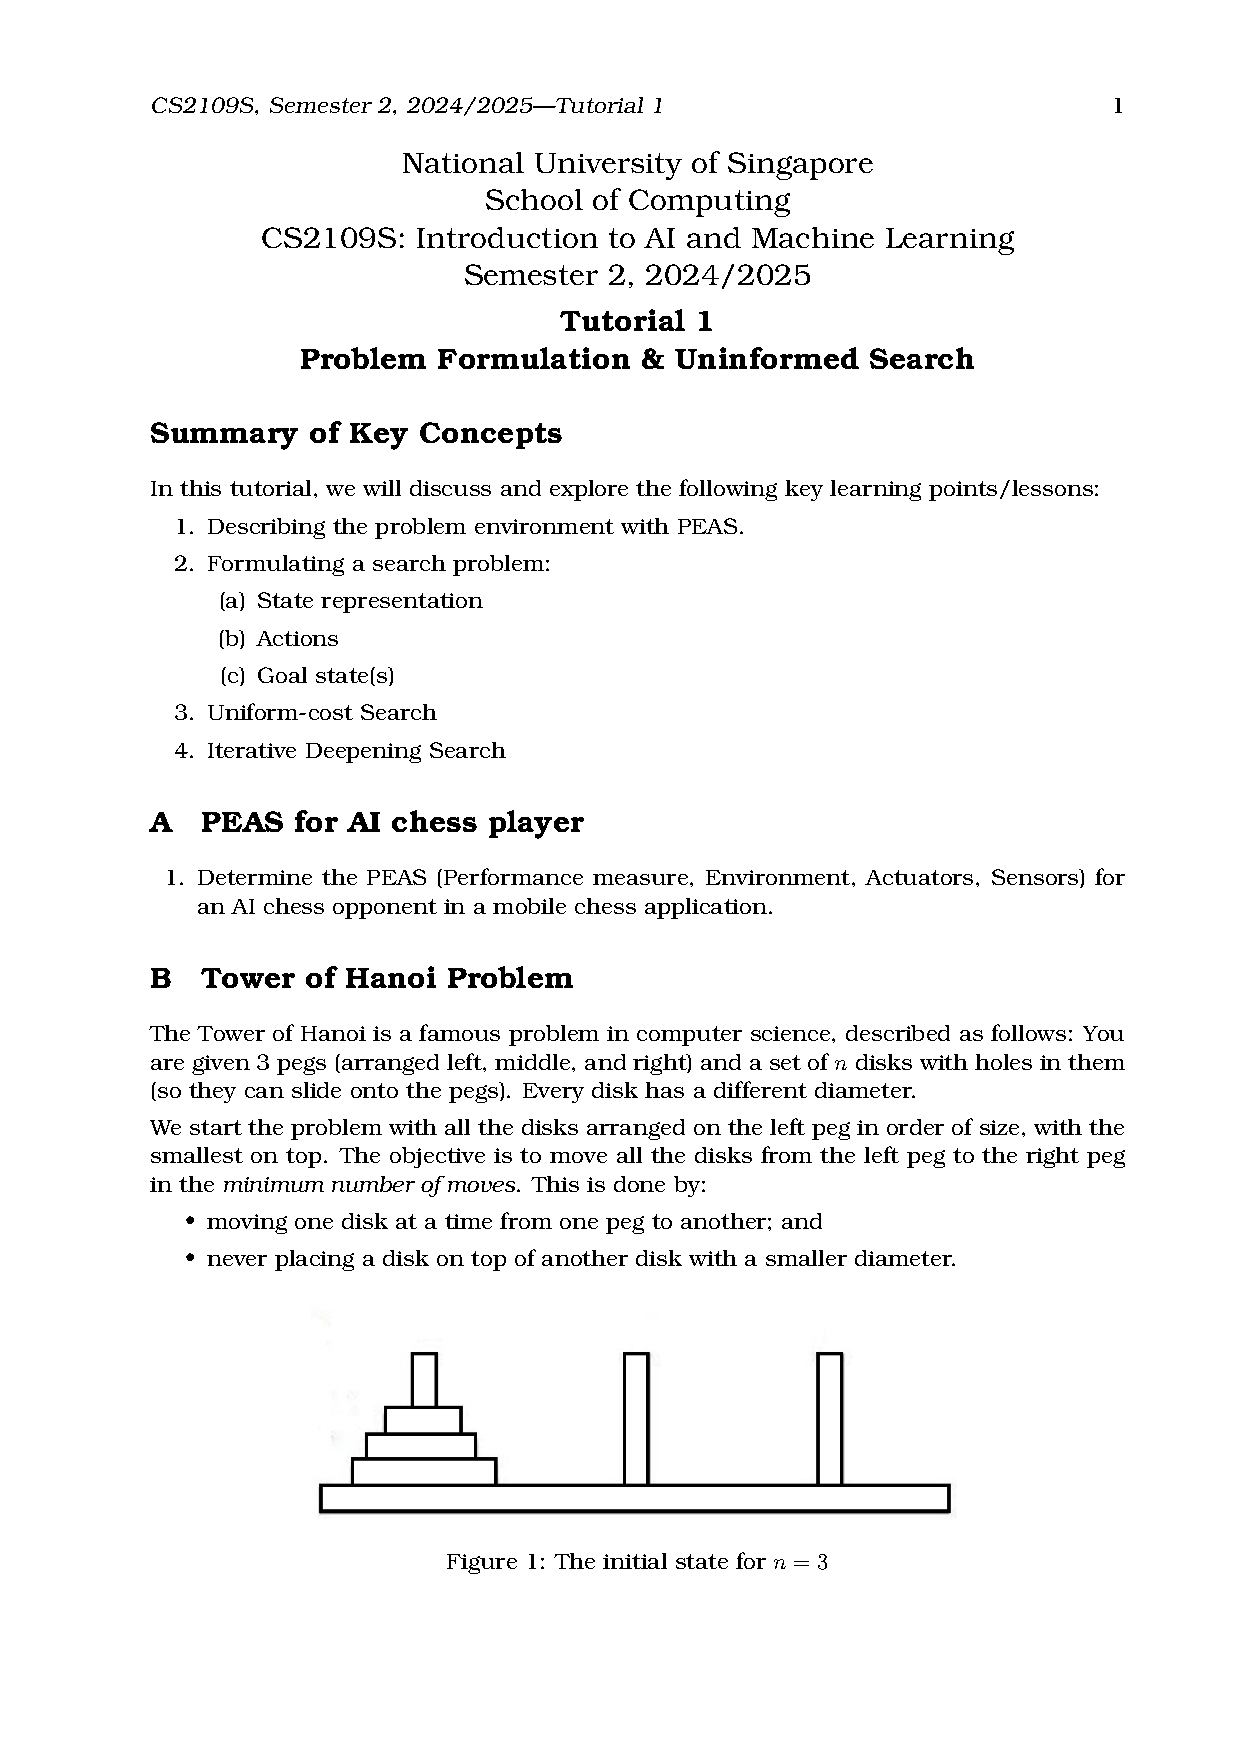
\includepdf[pages=1]{Tutorial1.pdf}
\section*{}
\subsection{}
\subsubsection*{a}
States: every possible placement scheme of all disks on all poles
Initial State: the starting placement of all disks
Goal States: placement scheme that satisfy the requirement
action: if $state_a$ can be transformed into $state_b$ my moving one disk, $state_b$ is reacheable from $state_a$ in cost 1 
\subsubsection*{b}
Representation invariant: No larger disk on smaller disks in all possible states
\subsection{}
Complete search. Hanoi tower is NP-hard thus the best general algorithm is of exponential complexity. To save memory, DFS may be used.
\subsection{}
$k - 1$. as there will be more choices of action from one state to another.
\includepdf[pages=2]{Tutorial1.pdf}
\section*{}

\includepdf[pages=3]{Tutorial1.pdf}
\section*{}

\includepdf[pages=4]{Tutorial1.pdf}
\section*{D}
\subsection{}
Linear search, or a tree search with braching factor 1, iterative deepening search perform in worse case scenario costs $O(n^2)$
while dfs costs $O(n)$
\subsection{}


\end{document}
